

\documentclass[10pt,a4paper]{article}
\usepackage[utf8]{inputenc}
\usepackage[spanish]{babel}
\usepackage{amsmath}
\usepackage{amsfonts}
\usepackage{amssymb}
\usepackage{graphicx}
\usepackage{lscape}

\begin{document}
\begin{large}
\begin{center}
\textbf{Diego Rosado Cabrera}\vspace{.3cm}

\textbf{Tecnologías, para el Internet}\vspace{.3cm}

\textbf{Tarea 01}
\end{center}
\end{large}

\begin{flushleft}
\section{Modelo Vista Controlador}

Primero recordemos que es el modelo vista controlador, , tomando en cuenta que este es un patrón de diseño que hará que dividamos nuestro programa en 3 partes principales los cuales son 

\begin{itemize}
\item[a] \textbf{Modelo :} Es aquel que va contener los datos y la funcionalidad de la aplicación

\item[b] \textbf{Vista } : Es el encargado de como se vería nuestra aplicación 

\item[c] \textbf{Controlador } : Es la encargada de manejar y responder las solicitudes del usuario , procesando la información necesaria que se necesita para que el programa funcione

    
\end{itemize}
Esto lo utilizamos , para que el código sea más legible  y además fácil de actualizar ya que de esta madera tiene una estructura mayormente legible.  

\section{Separación de clase }

\begin{flushleft}
Para poder hacer un buen modelo vista controlador separaremos nuestro programa en 10 diferentes clases para lograr un buen diseño 

\subsection{Vista}
 
Esta sección solo hablaremos de las 4 clases que conforman a la sección de vista 
\end{flushleft}

\begin{itemize}
\item[a] \textbf{Menú compras:} Esta clase unicamente se dedicara mostrar los precios de los productos que tenemos a la venta.  
\item[b] \textbf{carrito compras :} En esta clase se encargara de mostrar lo que hemos comprado hasta el momento en la parte de el menú 
\item[c] \textbf{confirmación compras:} Esta clase mostrara todo lo que se guardo en el carrito de compras y para preguntar por 
\item[d] \textbf{Ticket:} La ultima clase de esta sección lo único que hace es decir que su pago fue procesado y si quieren ver el seguimiento de su paquete 
\end{itemize}

\subsection{Modelo}

Esta sección consta de 3 clases las cuales son :
\begin{itemize}
\item[a] \textbf{Datos almacén}: Esta parte al ser parte de el modelo se dedica a que el usuario pueda hacer todas las operaciones como vacear el carro agregar cosas al caro de compra entre otras.
\item[b] \textbf{Creador cuenta}: En esta lo único que hacemos es recibir la información de todo lo que  se compro para poder hacer la cuenta final o regresarte al menú principal

\item[c] \textbf{cobro}: Sirve para poder verificar que todos los datos sean correctos para la compra. 
\end{itemize}

\subsection{Controlador}

Esta sección tiene las ultimas 3 clases que manejaremos para poder usar nuestro proyecto
\begin{itemize}
\item[a]\textbf{Almacén}: Esta clase su objetivo es poder guardar el número de objetos que tenemos y sus respectivos precios 	
\item[b]\textbf{Carro Compra clientes}: Sirve para que guarden todos los objetos, que el cliente ha decidido comprar  
\item[c]\textbf{Objeto}: Esta es un clase donde guardaremos el nombre de los objetos que deseamos y el precio que esto tiene 
\end{itemize}
\end{flushleft}



\newpage

\begin{landscape}

\begin{figure}
  \centering
    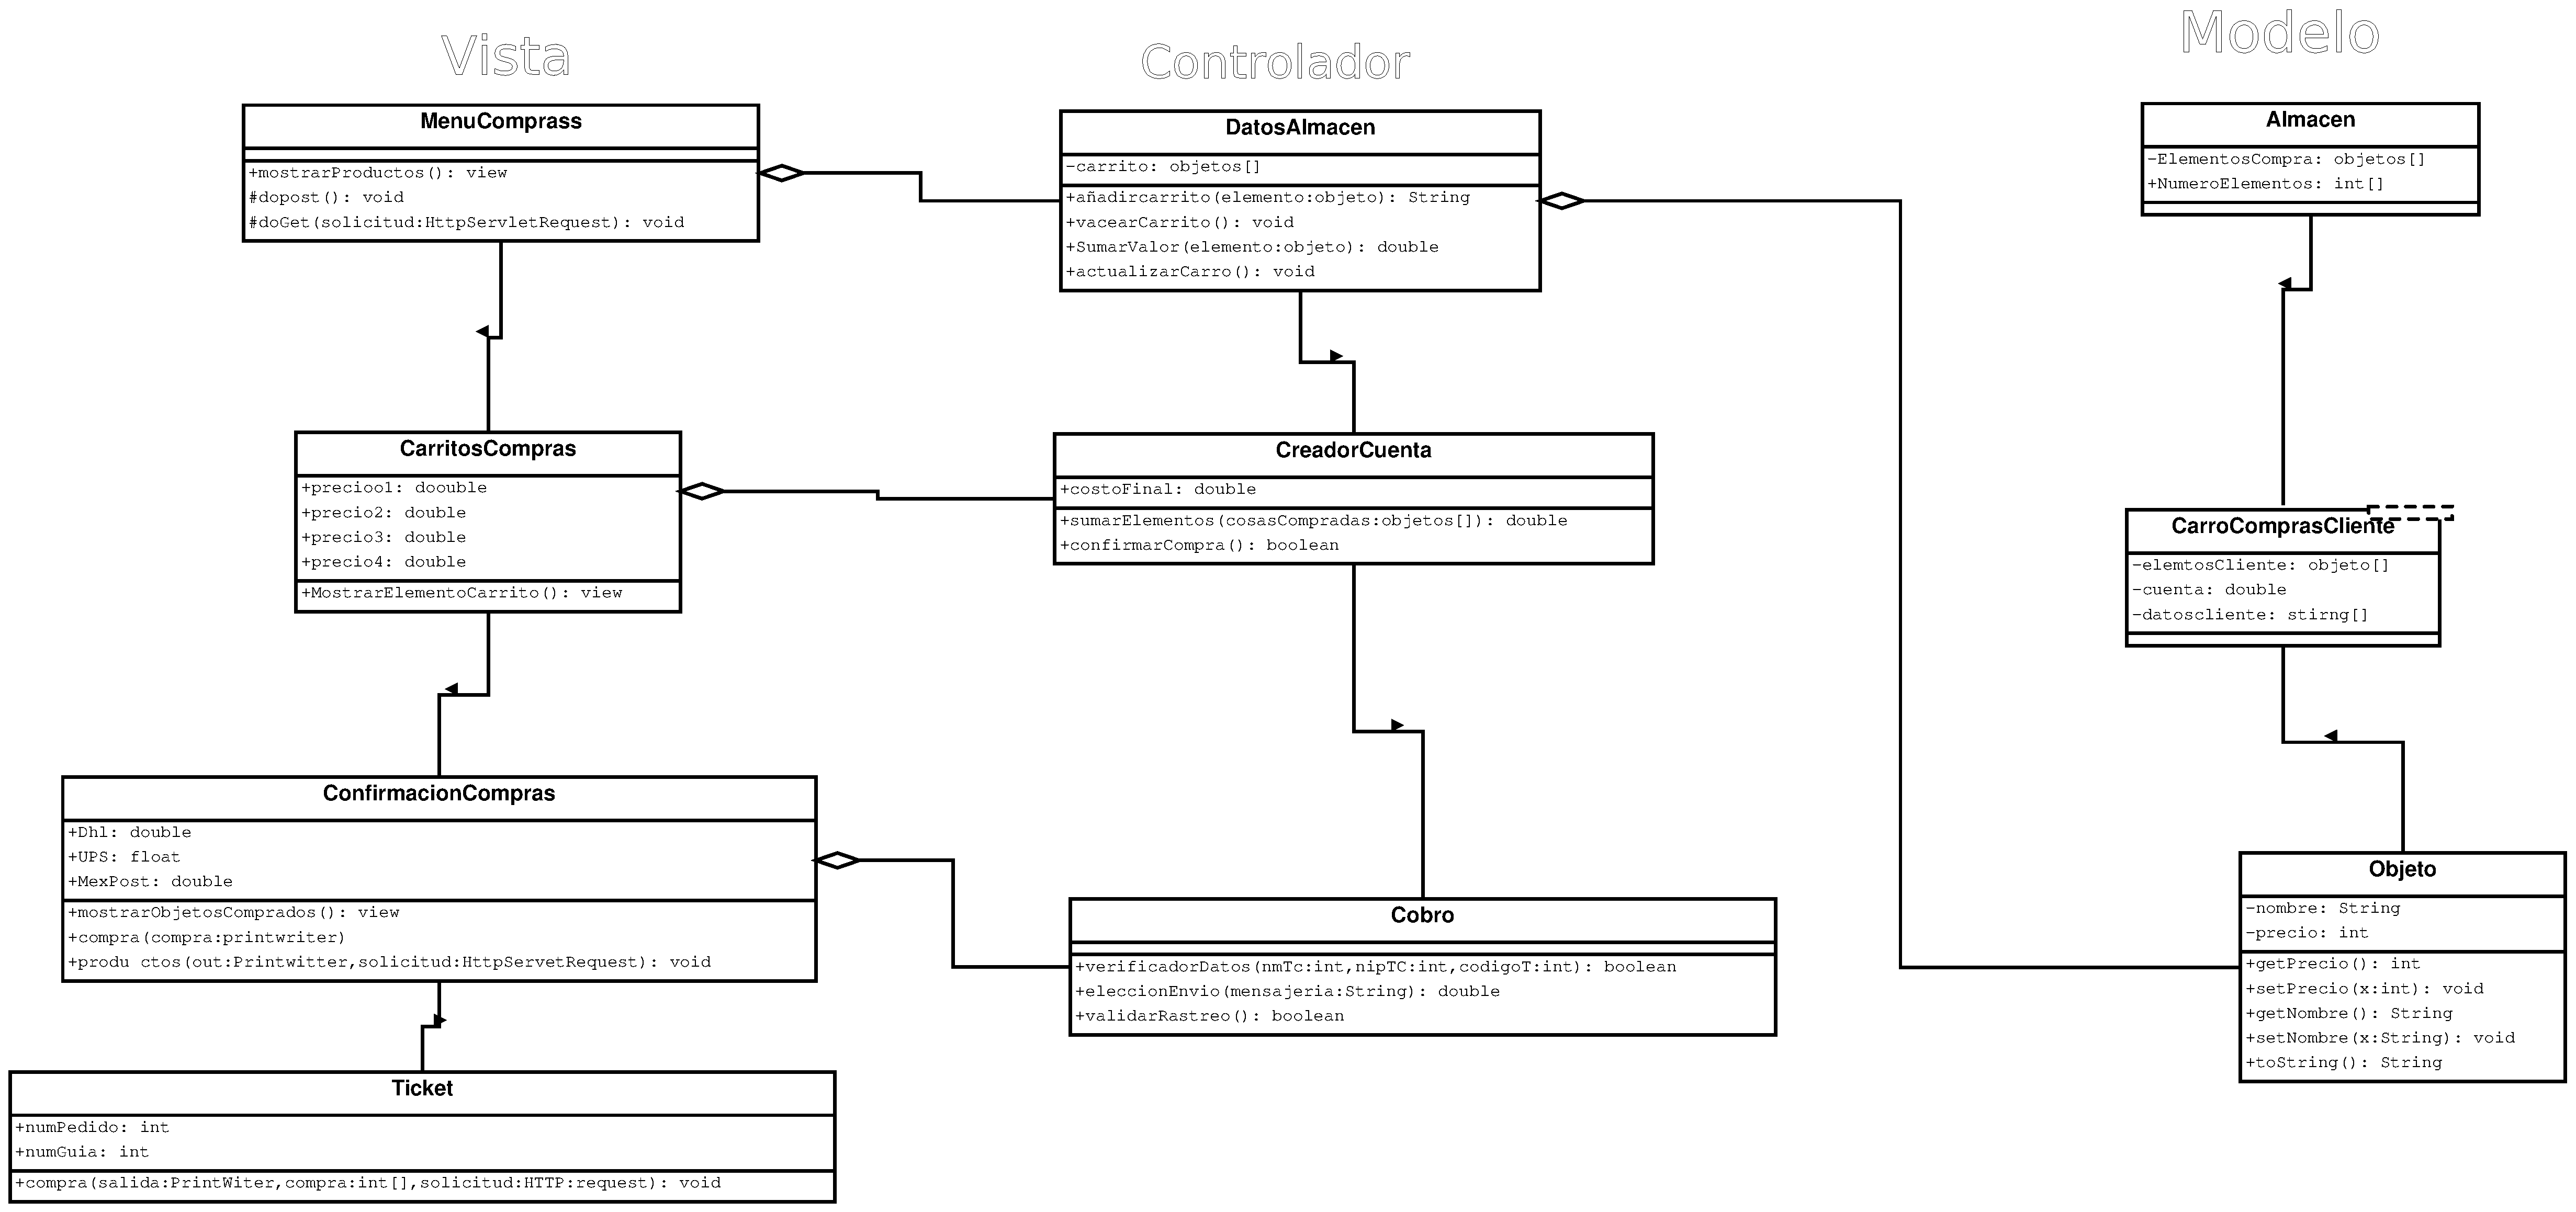
\includegraphics[width=2\textwidth]{Tarea1}
  \caption{Mi Figura}
  \label{fig:ejemplo}
\end{figure}
\end{landscape} 



\end{document}